\chapter{ESP8266 Development Board}

\section{Tujuan}
\begin{enumerate}
    \item Mempraktikkan teknik penyolderan SMD untuk membangun Development Board pada mikrokontroler ESP8266.
    \item Memahami karakteristik dan kebutuhan khusus dalam penyolderan komponen SMD.
    \item Mendapatkan keahlian dalam menangani alat solder untuk komponen elektronik ukuran kecil.
    \item Mengembangkan kemampuan untuk membaca skematik dan menerapkannya pada pembuatan prototipe elektronik.
    \item Memahami mekanisme cara menanamkan program ke ESP8266.
\end{enumerate}

\section{Dasar Teori}
Development Board ESP8266 merupakan papan pengembangan yang dirancang untuk memudahkan penggunaan mikrokontroler ESP8266. ESP8266 sendiri adalah mikrokontroler dengan kemampuan Wi-Fi dan Bluetooth terintegrasi yang sering digunakan untuk proyek IoT (Internet of Things). Dalam penyolderan ESP8266, komponen elektronik dipasang langsung ke permukaan PCB tanpa menggunakan kaki atau pin melalui lubang. 

Penyolderan SMD memerlukan presisi dan kecermatan karena ukuran komponen yang sangat kecil dan pad yang berdekatan satu sama lain. Penggunaan stencil dalam proses penyolderan SMD memungkinkan aplikasi pasta solder yang seragam dan akurat, yang sangat penting untuk mencegah short-circuit pada pad-pad yang berdekatan.

Proses penyolderan SMD untuk ESP8266 melibatkan langkah-langkah seperti penyiapan stencil, aplikasi pasta solder, penempatan komponen dengan pinset atau vacuum pickup tool, dan penyolderan menggunakan solder ujung halus atau hot air rework station. Pemeriksaan visual dan pengujian fungsional dilakukan setelah penyolderan untuk memastikan kualitas sambungan dan fungsi rangkaian secara keseluruhan.

\section{Tugas Pendahuluan}
\begin{enumerate}
    \item Install Visual Studio Code 
    \item Install ekstensi PlatformIO pada Visual Studio Code 
    \item Download firmware dari \url{https://intip.in/WortelBoardGn24} lalu build project menggunakan vscode + Platformio sampai sukses
    \item Bukalah \url{https://intip.in/TupenWortelP4} berikut lalu buat program untuk menghidupkan lampu ketika tombol ditekan

\end{enumerate}

\section{Alat dan Komponen}
\subsection{Alat}
\begin{enumerate}
    \item Soldering kit
    \item Timah 0.8 mm
    \item Power source
    \item Sikat 
    \item IPA (Isopropyl alcohol)
    \item Flux
    \item Solder Pasta
    \item Stencil Holder
    \item Stencil
    \item Multimeter
    \item USB to TTL
\end{enumerate}

\subsection{Komponen}
\begin{enumerate}
    \item Development Board ESP8266 Kit
\end{enumerate}

\section{Eksperimen 1: Stencil dan Aplikasi Pasta Solder}
\begin{center}
    \colorbox{gray}{\parbox{0.8\linewidth}{\textbf{Disclaimer:} Board yang digunakan di modul dan saat praktikum akan memiliki sedikit perbedaan. Namun secara garis besar, caranya hampir sama.}}
\end{center}
\begin{enumerate}
    \item Siapkan stencil dan pasta solder.
    \item Posisikan pcb di atas stencil holder.
    \begin{figure}[H]
        \centering
        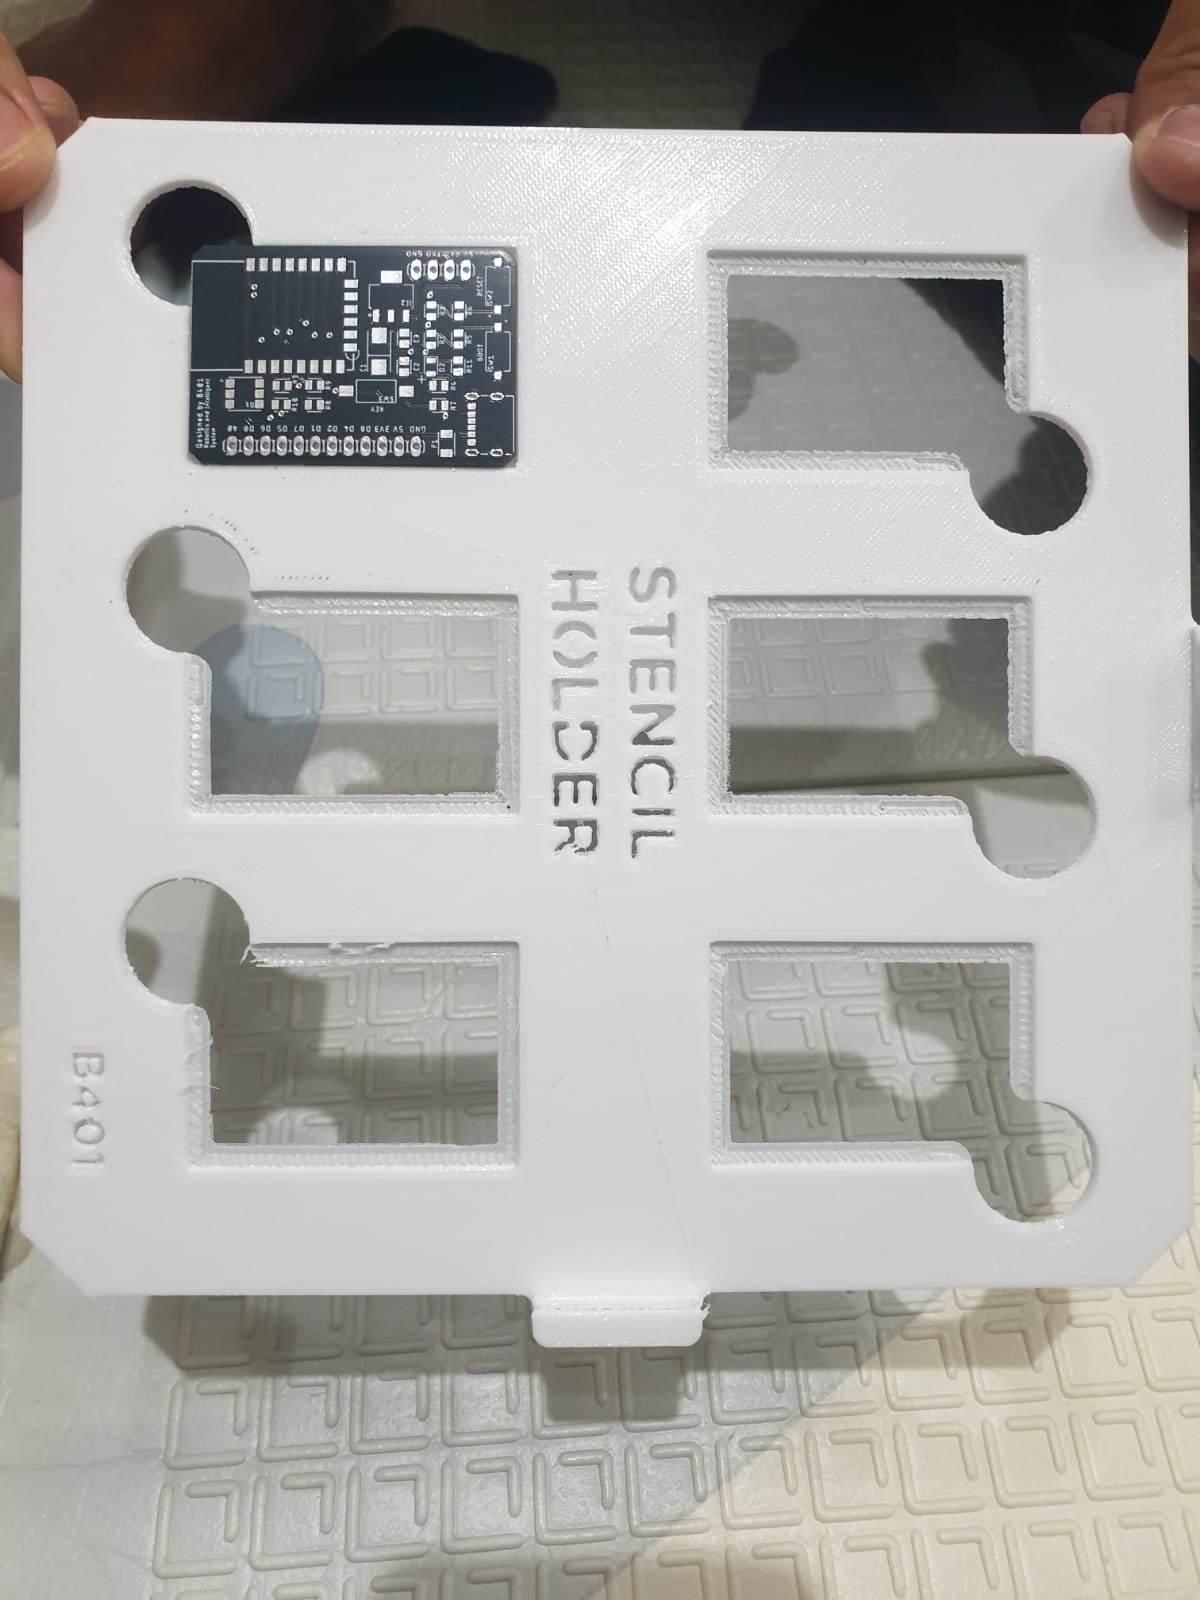
\includegraphics[width=0.4\linewidth]{P4/img/1_board_minsys_ke_holder_stencil.jpeg}
        \caption{Penempatan Board di Stencil}
        \label{fig:PenempatanBoarddiStencil}
    \end{figure}
    \item Letakkan stencil di atas PCB dan pastikan posisi stencil tepat di atas pad.
    \begin{figure}[H]
        \centering
        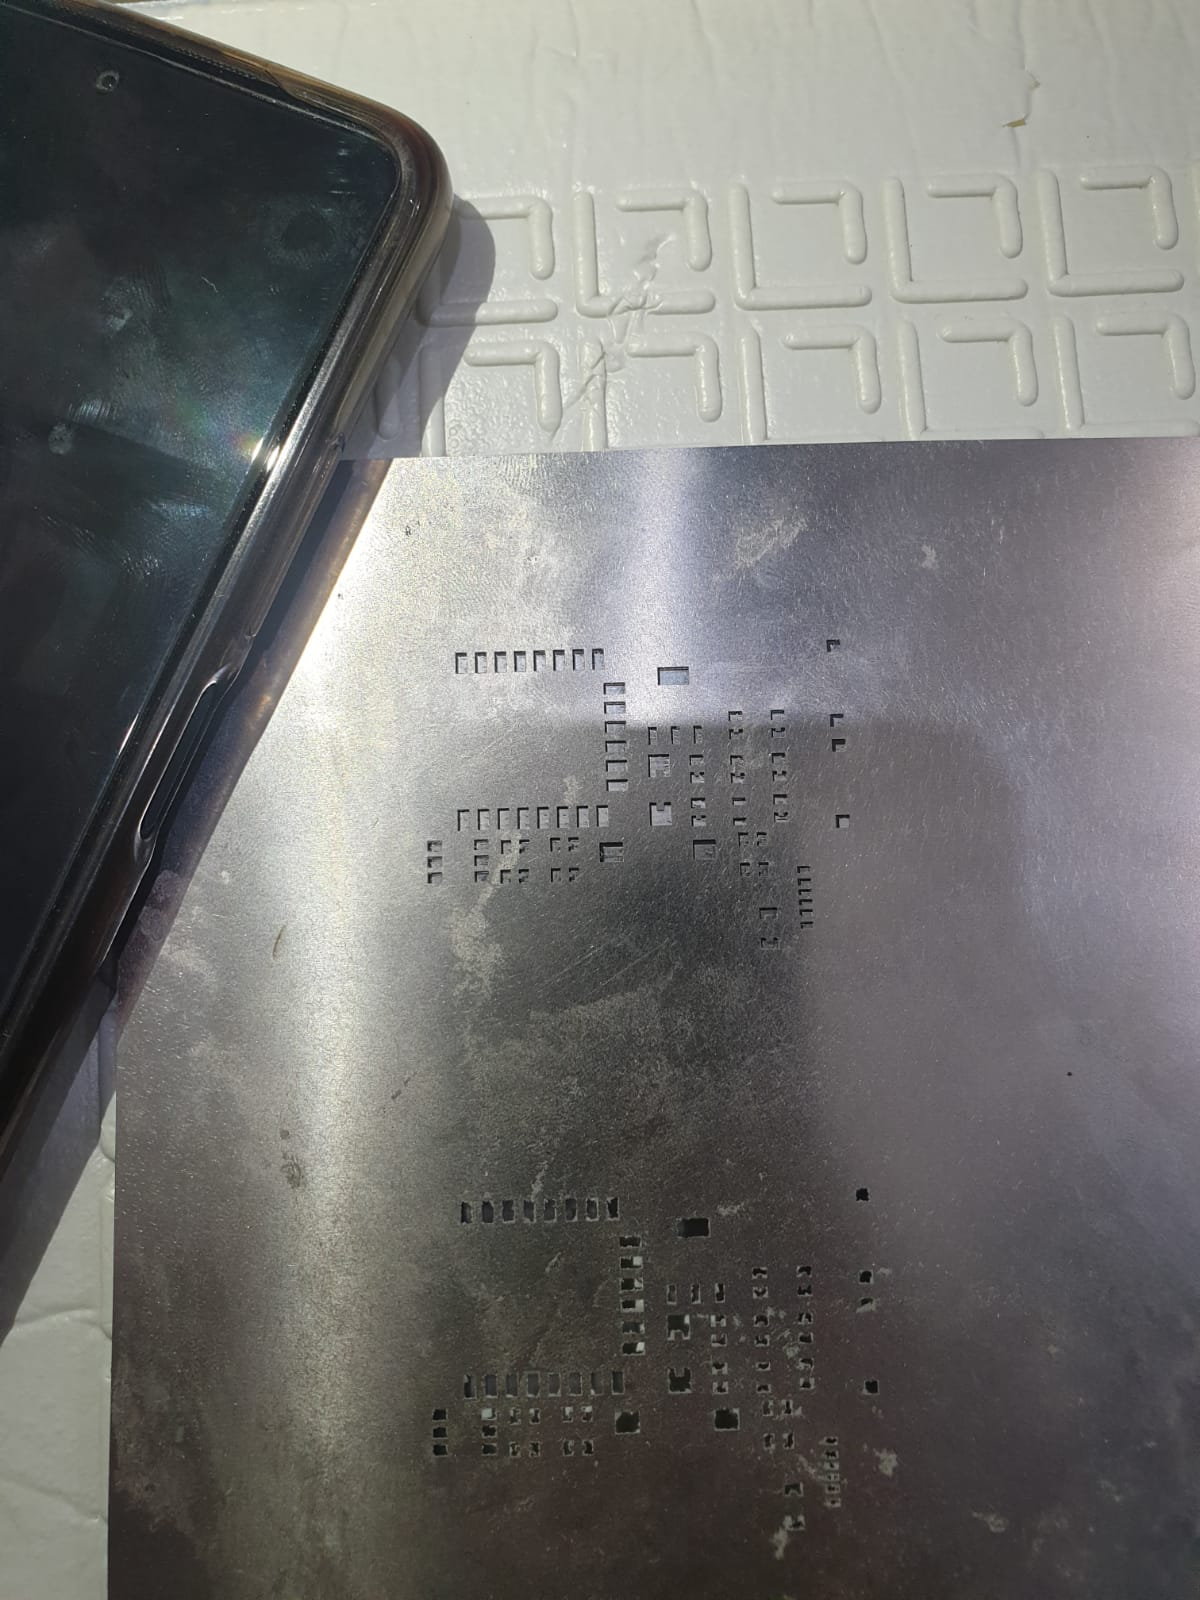
\includegraphics[width=0.4\linewidth]{P4/img/2_pastikan_stencil_pas.jpeg}
        \caption{Stencil Tepat di Atas Pad}
        \label{fig:StencilTepatdiAtasPad}
    \end{figure}
    \item Tuangkan solder pasta ke stencil.
    \begin{figure}[H]
        \centering
        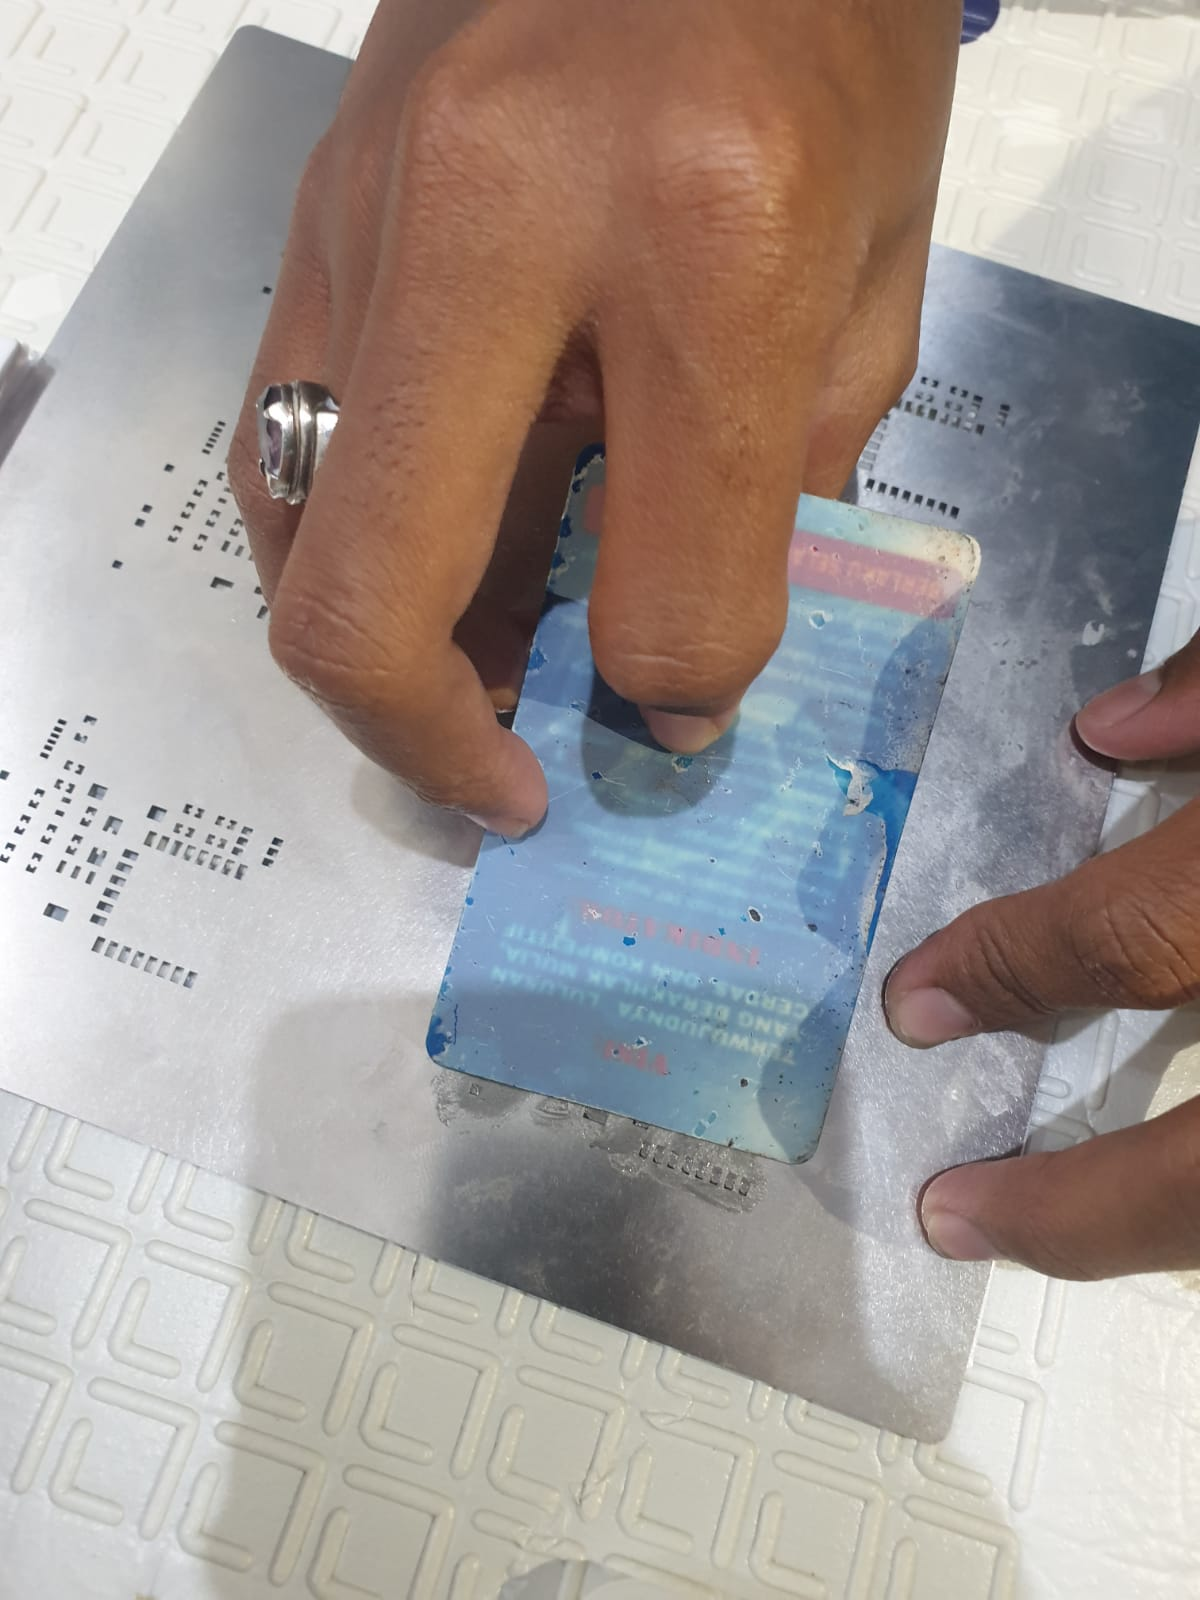
\includegraphics[width=0.4\linewidth]{P4/img/3_taruh_solder_pasta_lalu_ratakan.jpeg}
        \caption{Taruh Pasta Solder}
        \label{fig:TaruhPastaSolder}
    \end{figure}
    \item Ratakan dengan menggunakan spatula.
    \item Bersihkan sisa pasta solder pada stencil.
    \item Periksa hasil aplikasi pasta solder pada PCB.
    \begin{figure}[H]
        \centering
        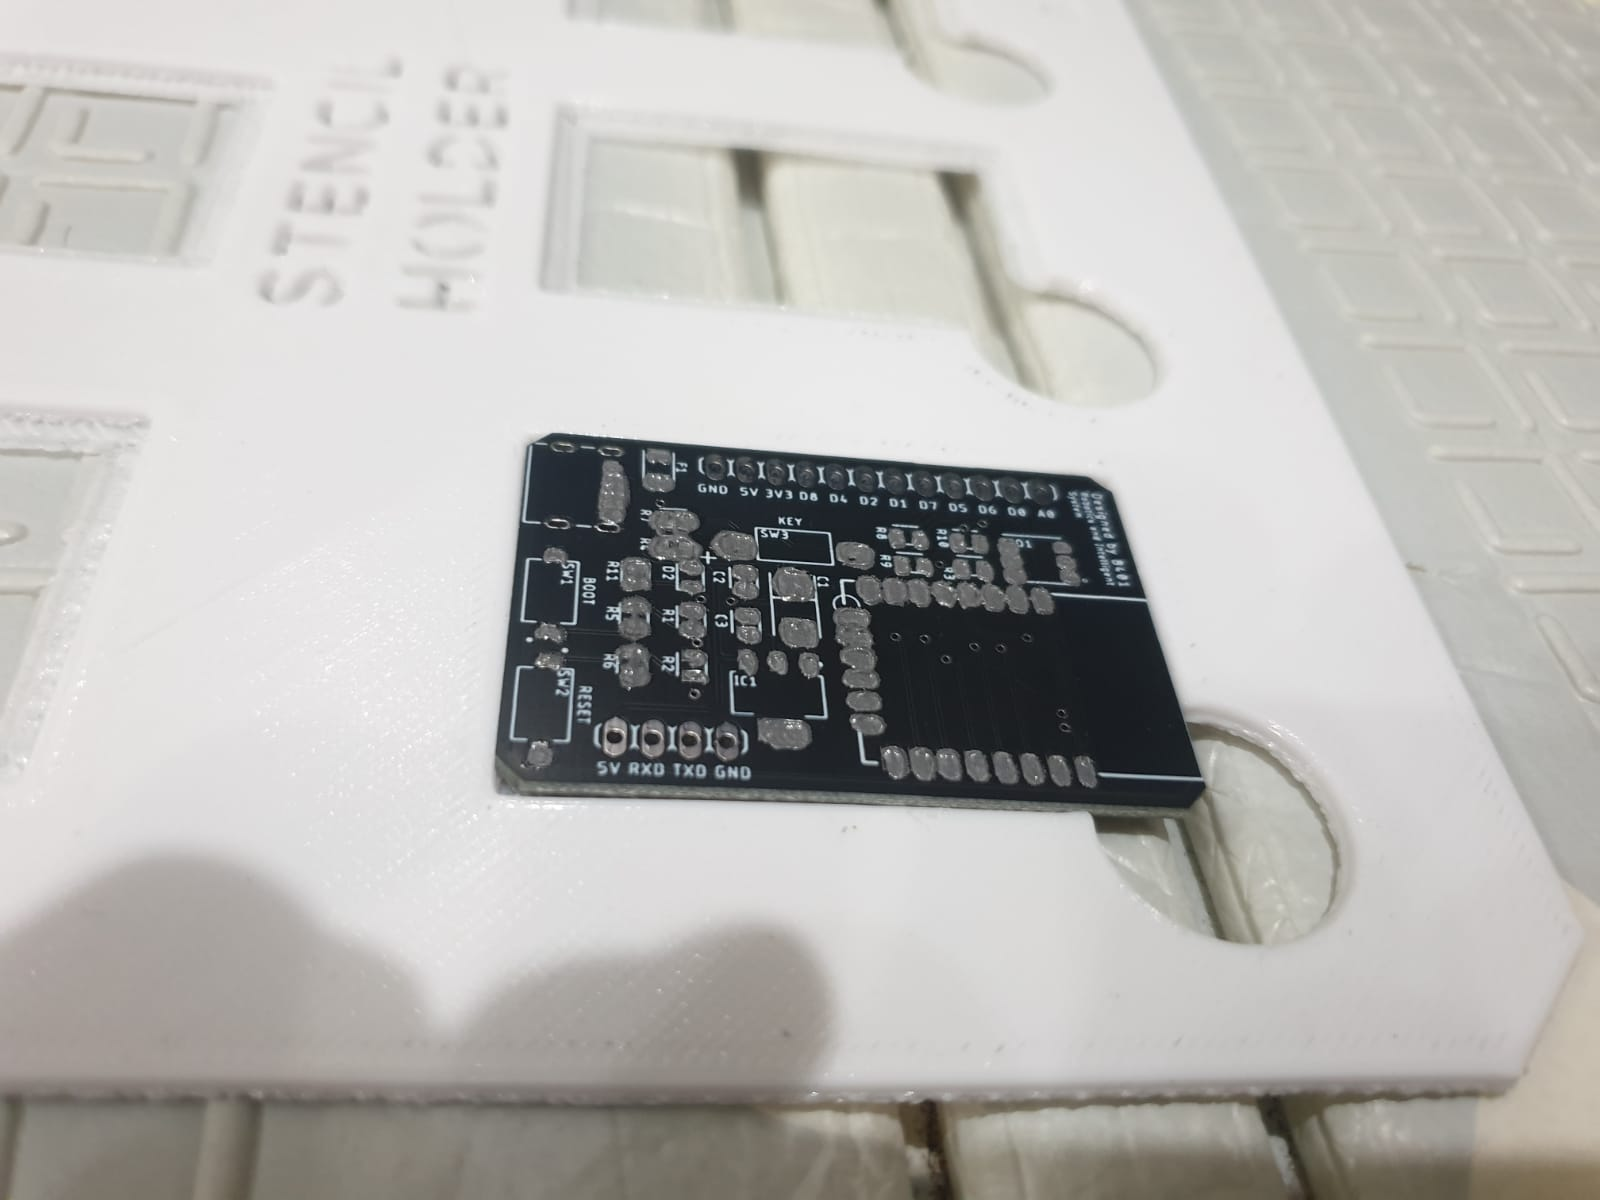
\includegraphics[width=0.4\linewidth]{P4/img/4_keadaan_board_setelah_dipasang_pasta.jpeg}
        \caption{Keadaan Board Setelah Dipasang Pasta}
        \label{fig:KeadaanBoardSetelahPasta}
    \end{figure}
    \item Angkat stencil dari stencil holder.
    \item Lepaskan PCB dari stencil holder dan pastikan solder pasta sudah sesuai dengaan pad PCB.
\end{enumerate}

\section{Eksperimen 2: Penempatan Komponen dan Penyolderan}
\begin{center}
    \colorbox{gray}{\parbox{0.8\linewidth}{\textbf{Disclaimer:} Board yang digunakan di modul dan saat praktikum akan memiliki sedikit perbedaan. Namun secara garis besar, caranya hampir sama.}}
\end{center}
\begin{enumerate}
    \item Siapkan komponen yang akan disolder.
    \item Buka dokumentasi Github \url{https://intip.in/WortelBoardGn24} folder hardware untuk melihat posisi komponen.
    \item Letakkan komponen SMD pada PCB sesuai dengan posisi mengikuti dokumentasi.
    \begin{center}
        \colorbox{pink}{\parbox{0.8\linewidth}{\textbf{Catatan:} Perhatikan posisi positif dan negatif pada komponen polar.}}
    \end{center}
    
    \item Setelah semua komponen diletakkan, periksa kembali posisi komponen.
    \begin{figure}[H]
        \centering
        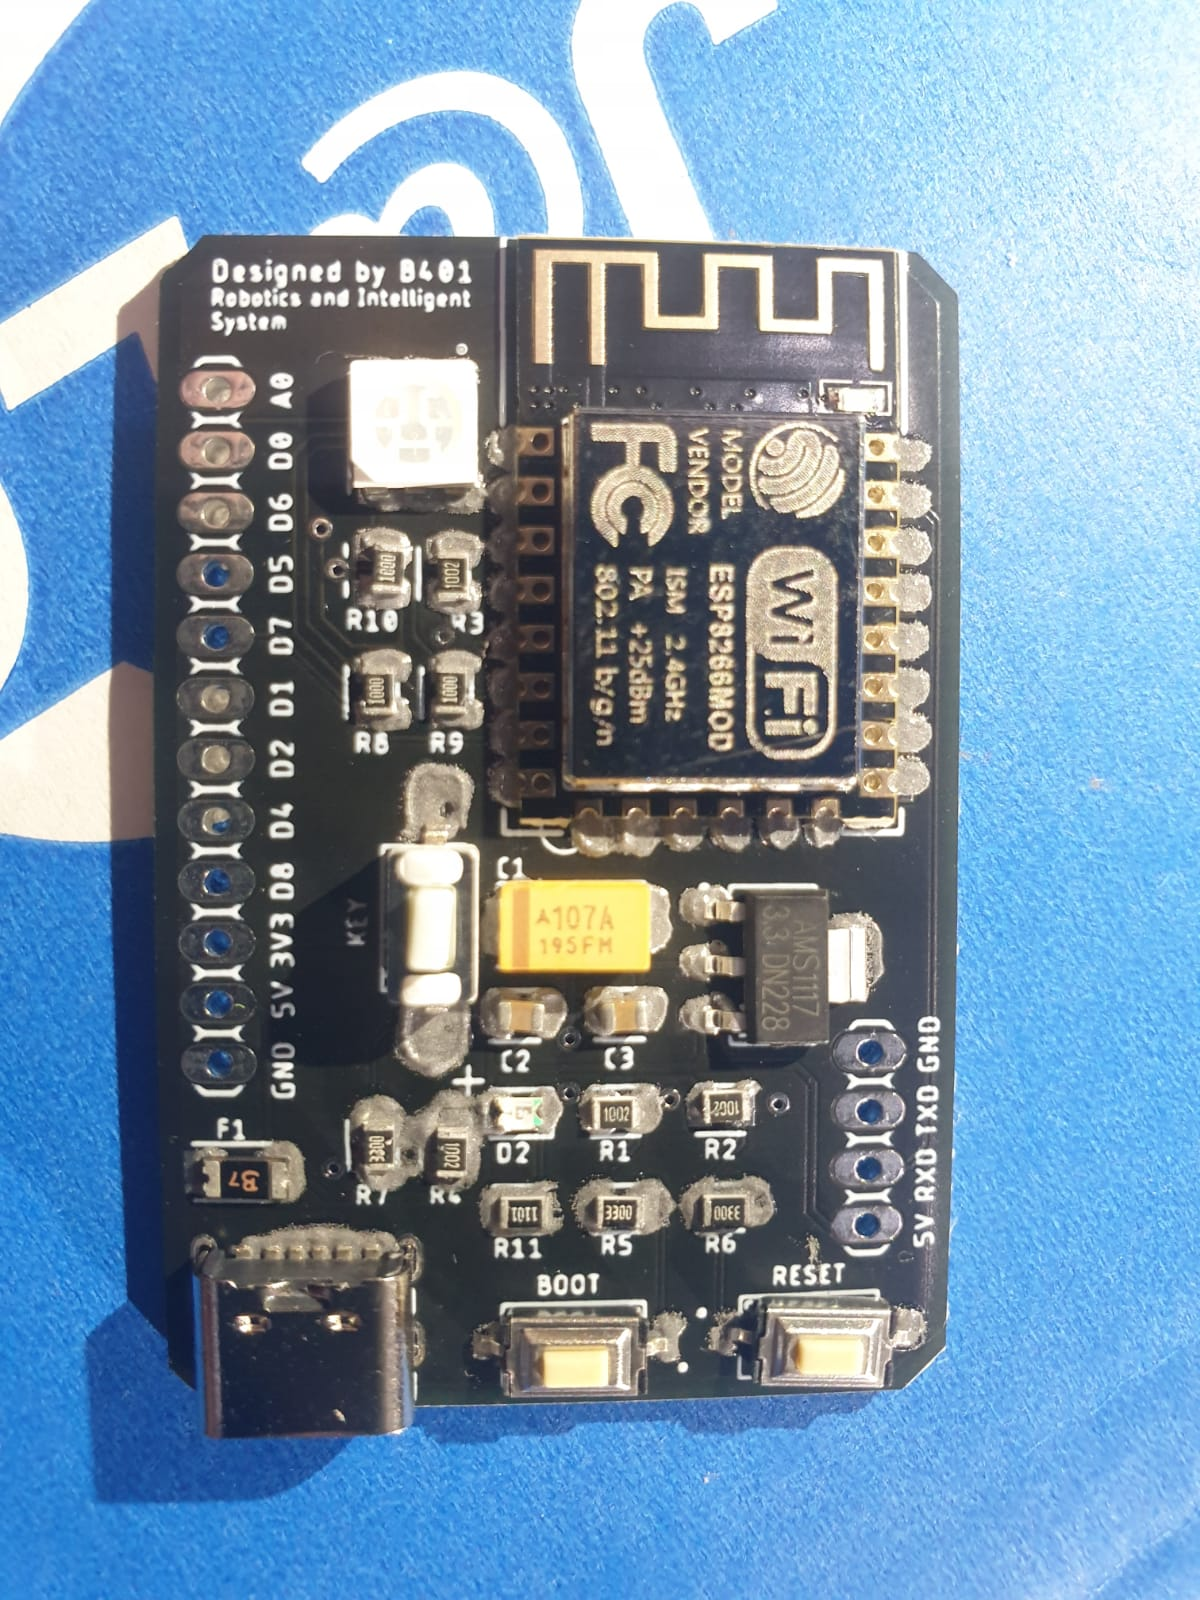
\includegraphics[width=0.4\linewidth]{P4/img/5_tampilan_board_ketika_sudah_dipasang_komponen.jpeg}
        \caption{Tampilan Board Setelah Dipasang Komponen}
        \label{fig:KeadaanBoardSetelahDipasangKomponen}
    \end{figure}
    \item Siapkan solder uap.
    % \begin{figure}[H]
    %     \centering
    %     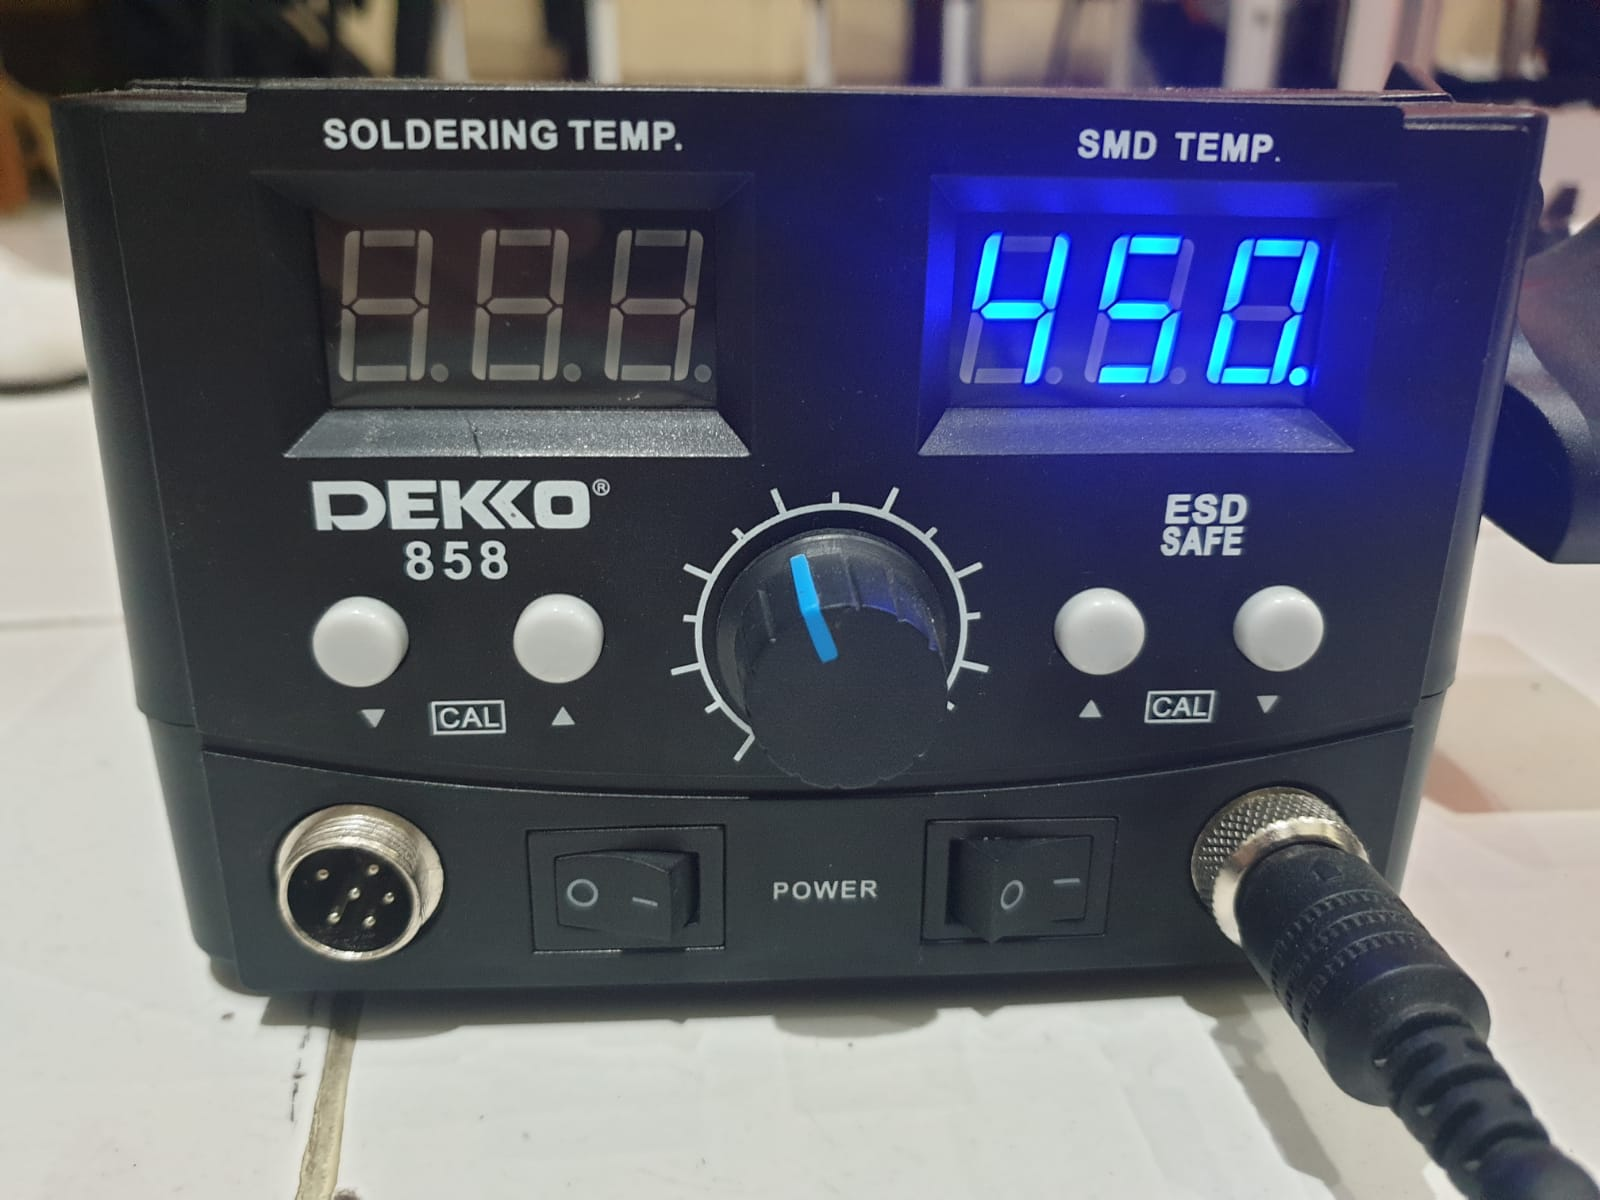
\includegraphics[width=0.4\linewidth]{P4/img/6_pastikan_switch_solder_uap_on_dan_suhu_standart_450.jpeg}
    %     \caption{Solder Uap On dan Suhu Standart 450$^{\circ}$C}
    %     \label{fig:SolderUapOn}
    % \end{figure}
    \item Solder komponen satu per satu dengan cara dekatkan ujung solder uap ke komponen hingga komponen menempel pada pcb. Pastikan kompone mengering sebelum berpindah ke komponen yang lain.
    \begin{center}
        \colorbox{pink}{\parbox{0.8\linewidth}{\textbf{Tips:} Solder komponen ESP8266 terlebih dahulu.}}
    \end{center}
    \begin{figure}[H]
        \centering
        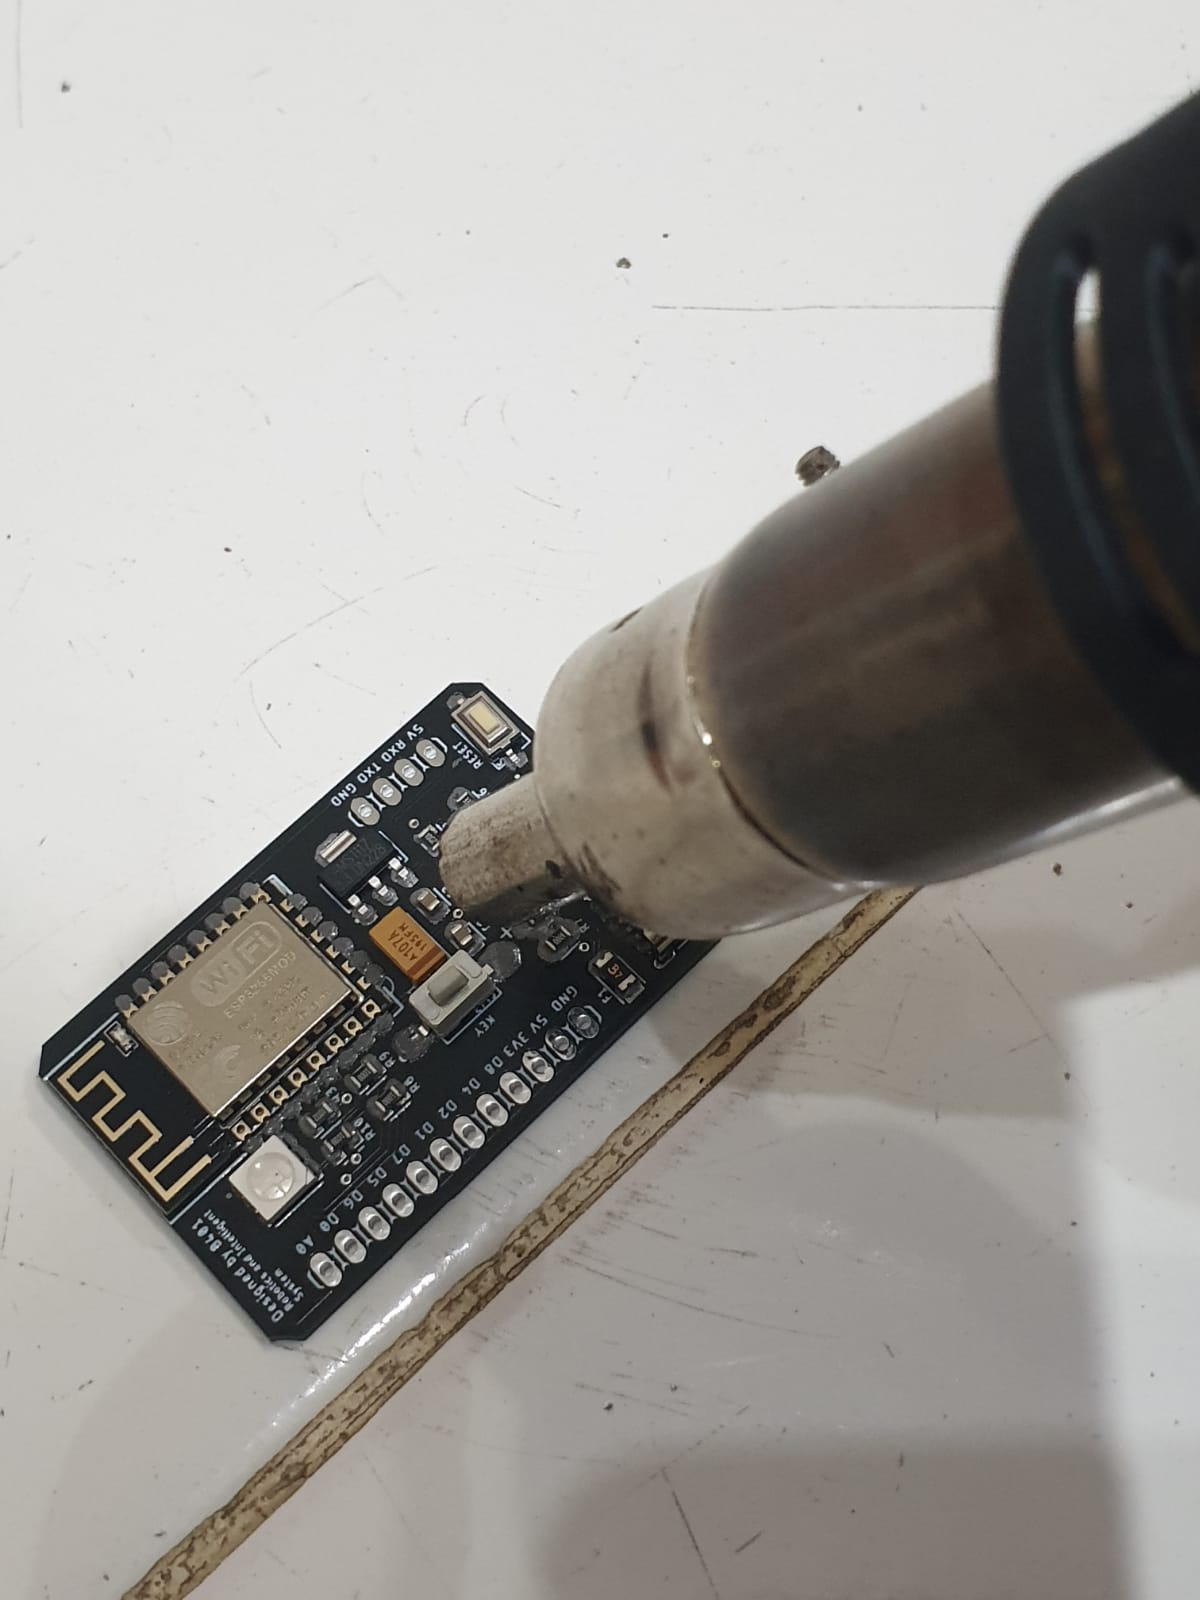
\includegraphics[width=0.4\linewidth]{P4/img/7_posisi_solder_uap_yang_benar.jpeg}
        \caption{Posisi Solder Uap}
        \label{fig:Posisi Solder Uap}
    \end{figure}
    \item Jika sudah selesai pastikan semua komponen sudah terpasang dengan baik.
    \begin{figure}[H]
        \centering
        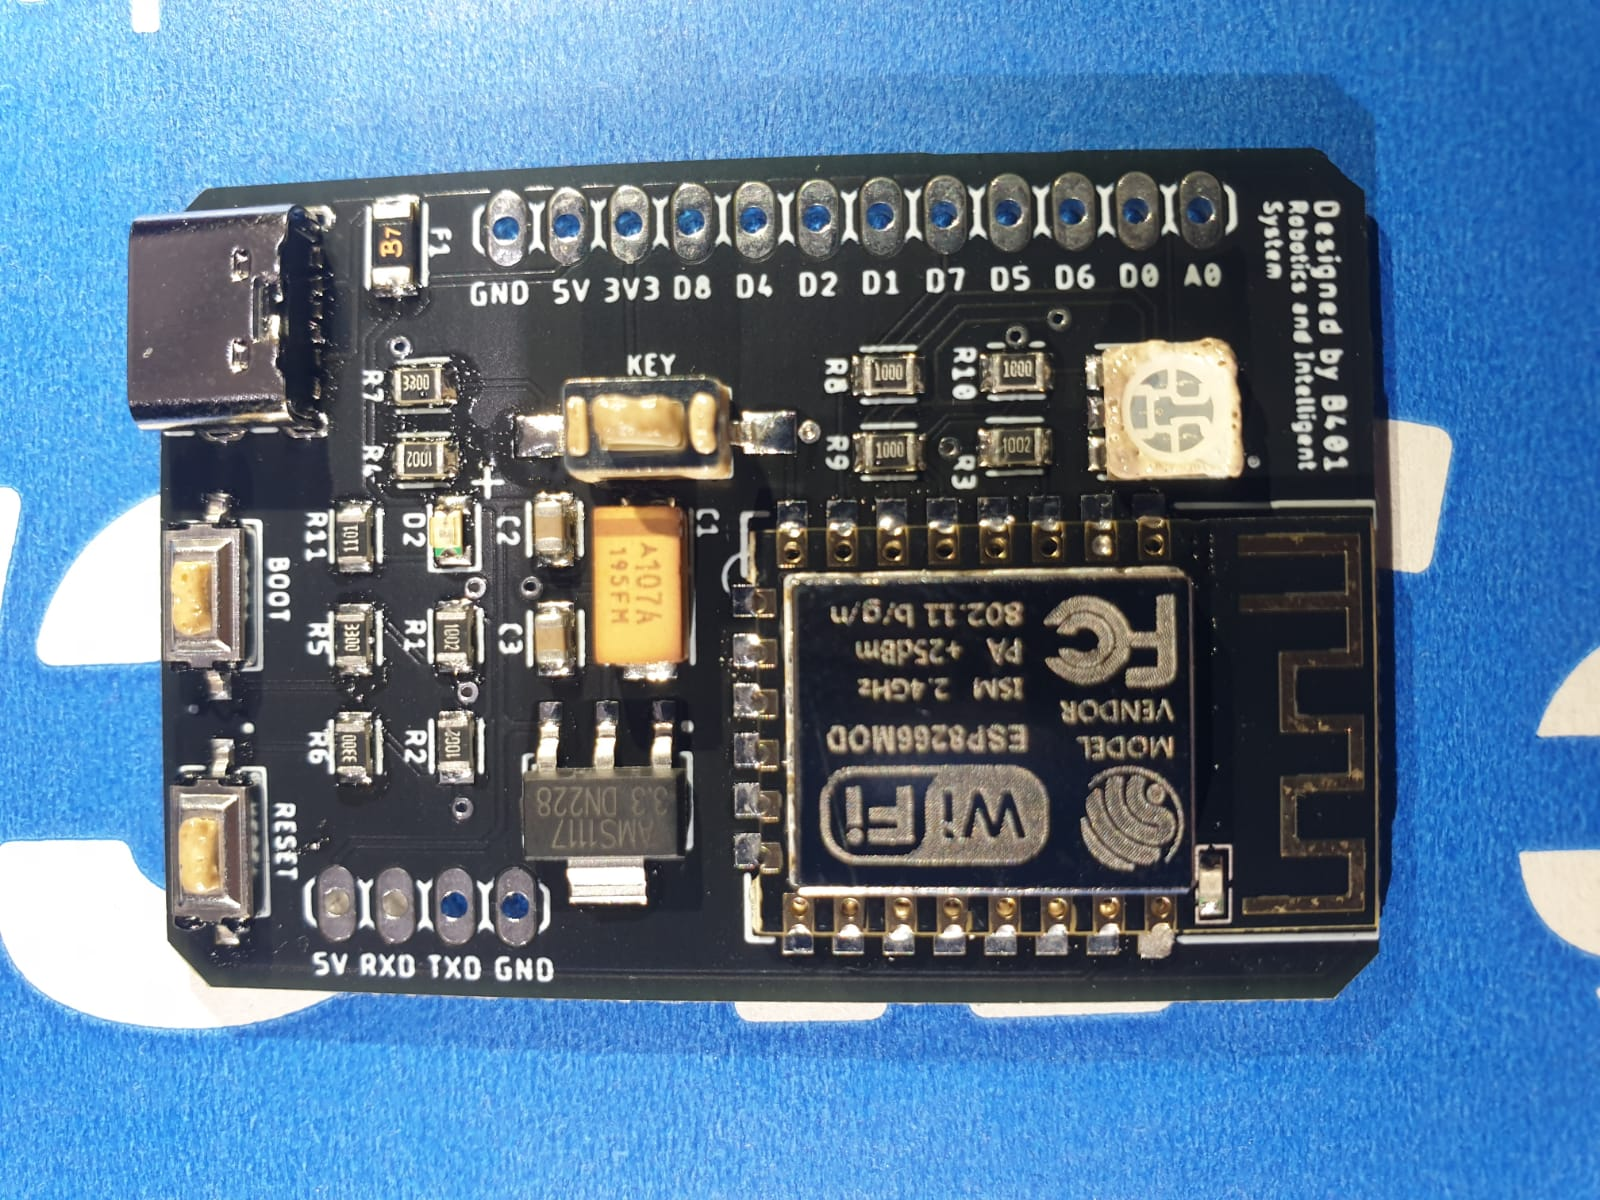
\includegraphics[width=0.4\linewidth]{P4/img/8_keadaan_board_full_komponen.jpeg}
        \caption{Keadaan Board Setelah di Solder}
        \label{fig:KeadaanBoardSetelahSolder}
    \end{figure}
    \item Solder pin header/true hole component dengan timah.
    \begin{figure}[H]
        \centering
        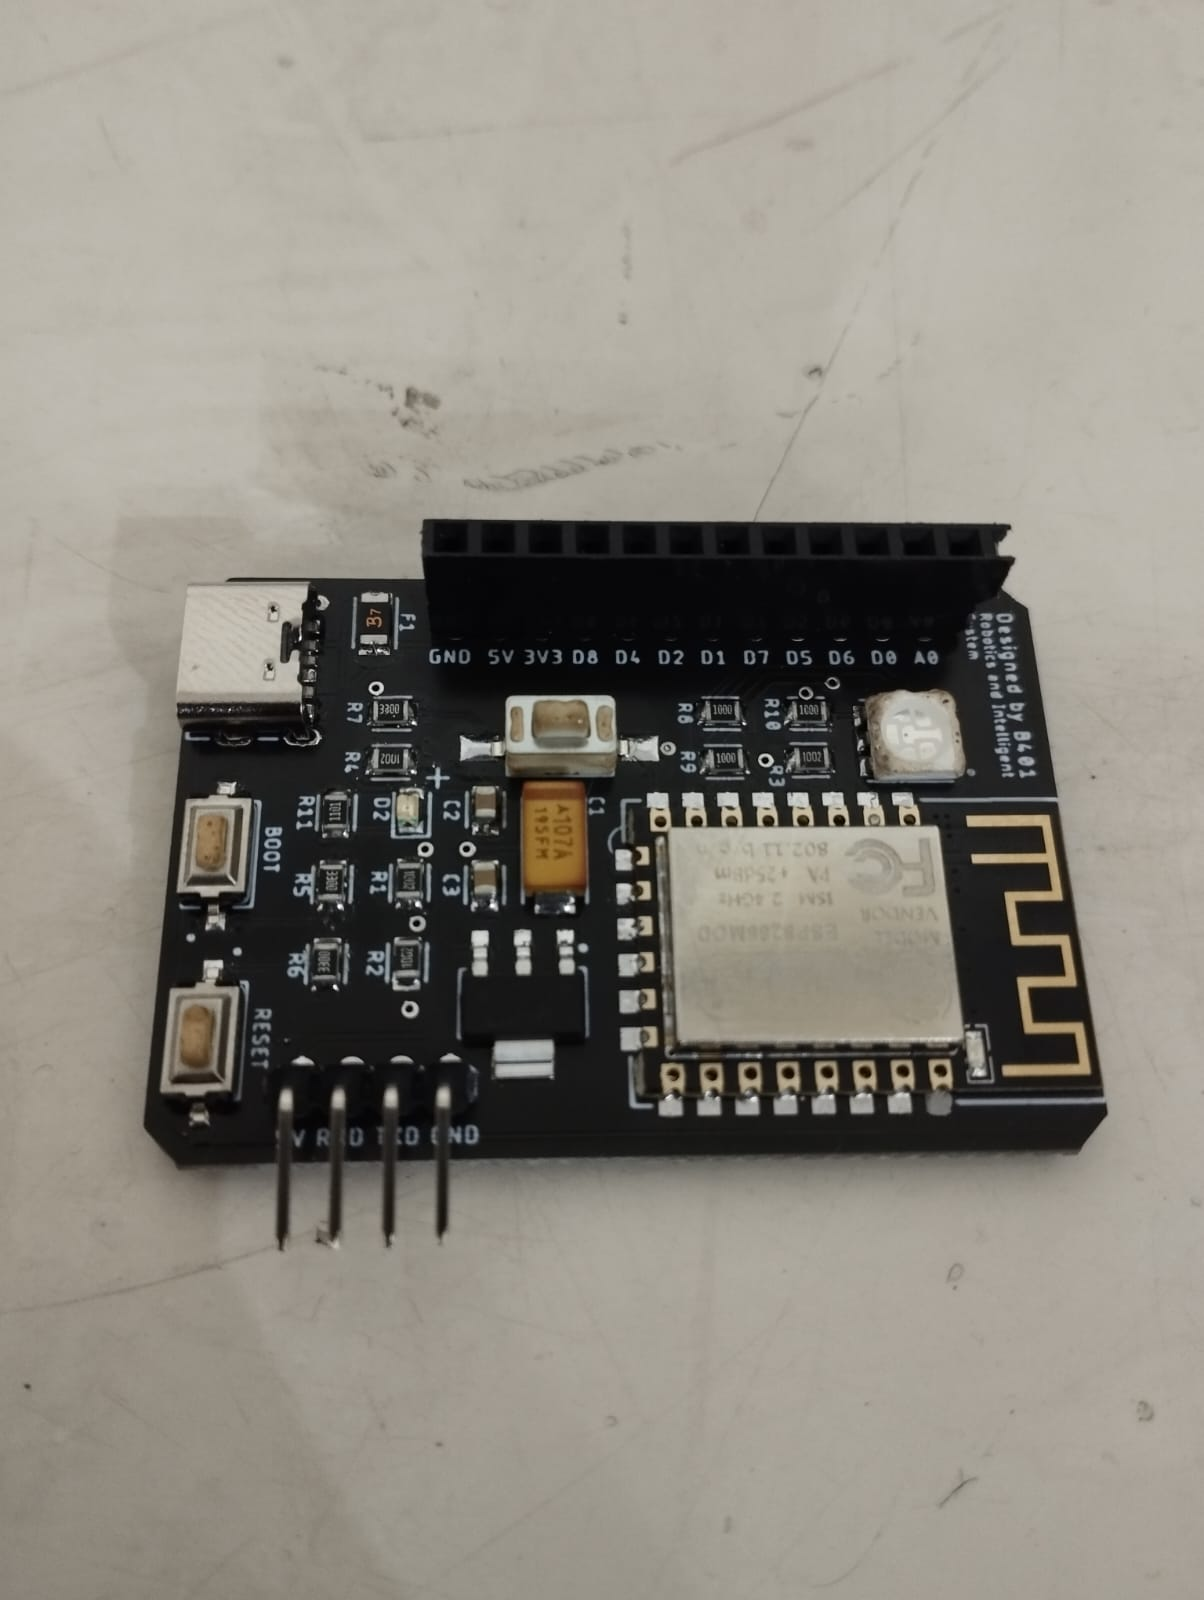
\includegraphics[width=0.4\linewidth]{P4/img/9_keadaan_setelah_disolder_headernya.jpeg}
        \caption{Keadaan Board Setelah Solder Header Pin}
        \label{fig:KeadaanBoardSetelahSolderHeader}
    \end{figure}
\end{enumerate}

\section{Eksperimen 3: Upload Firmware dan Pengujian Fungsional}
\begin{enumerate}
    \item Siapkan modul USB to TTL.
    \item Hubungkan modul ke komputer dan Development Board ESP8266.
    \subitem 5V TTL -> 5V ESP8266
    \subitem Tx TTL -> Rx ESP8266
    \subitem Rx TTL -> Tx ESP8266
    \subitem Gnd TTL -> Gnd ESP8266
    \begin{figure}[H]
        \centering
        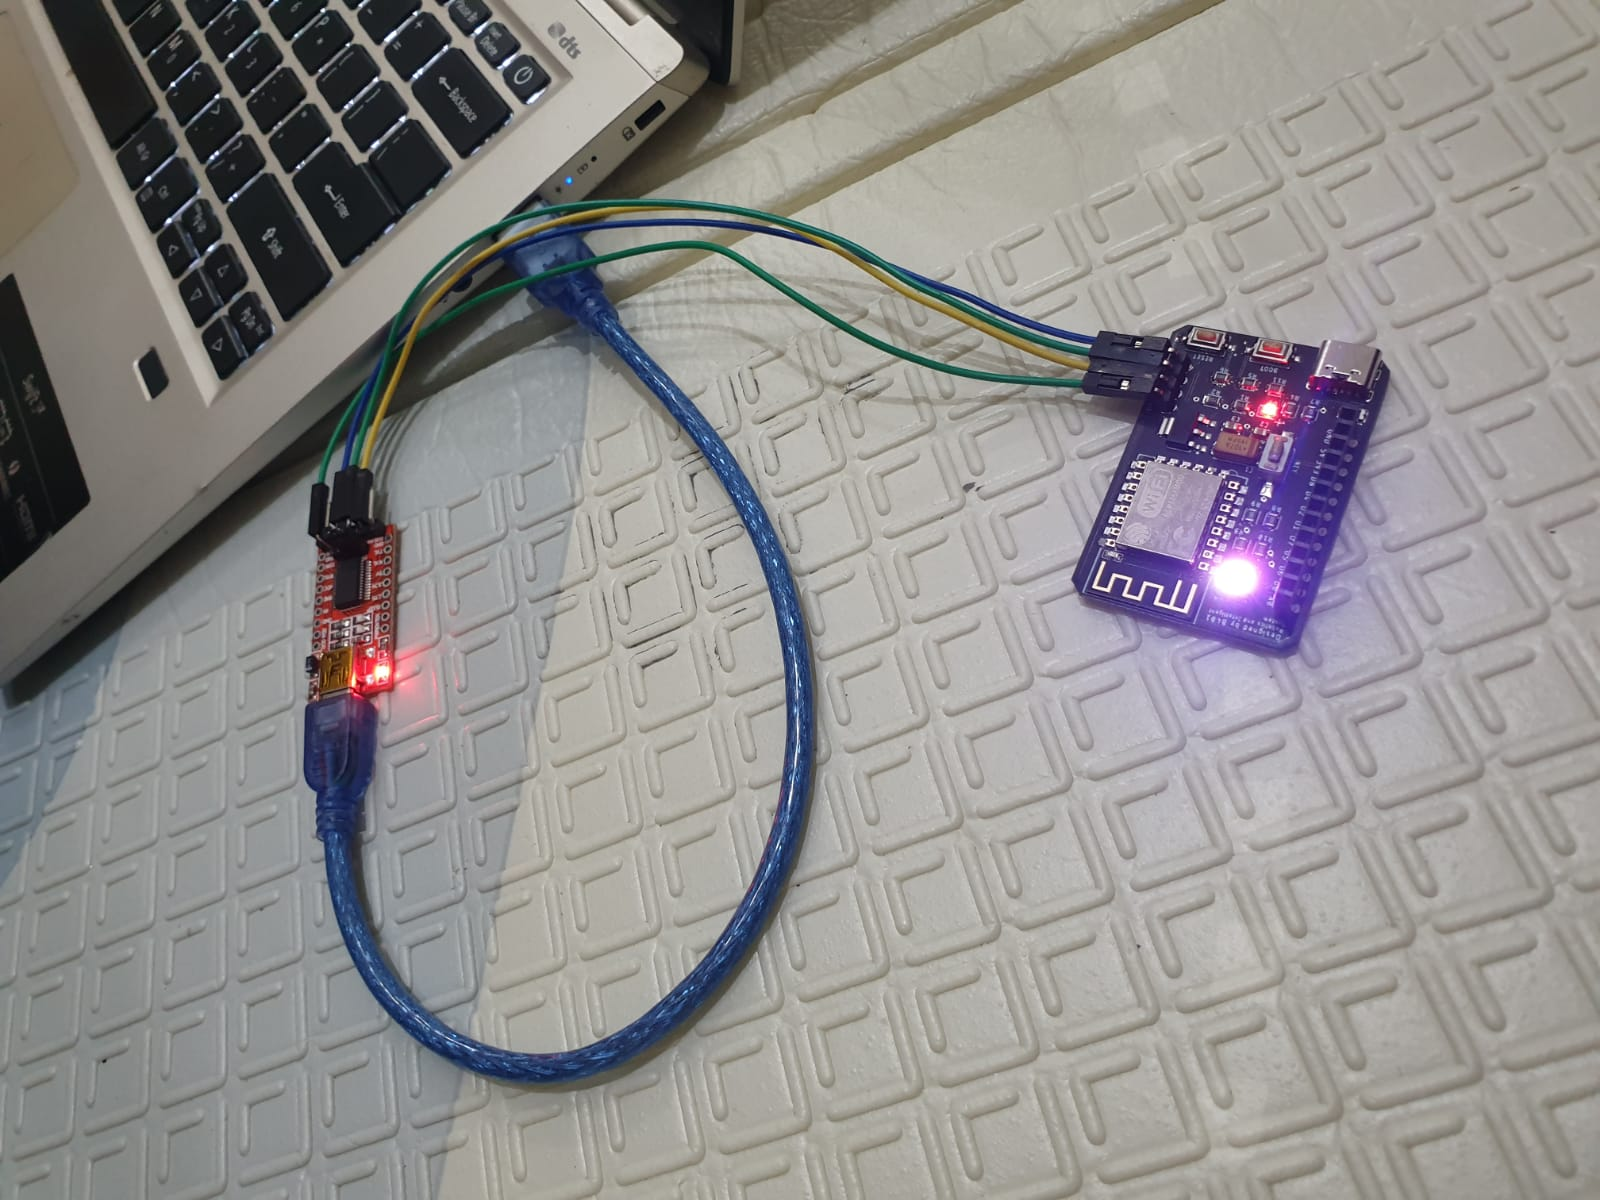
\includegraphics[width=0.4\linewidth]{P4/img/10_hubungkan_dengan_usbttl_dan_laptop.jpeg}
        \caption{USBTTL Dihubungkan ke Laptop}
        \label{fig:USBTTLLaptop}
    \end{figure}
    \item Bukalah subfolder firmware pada folder project yang sudah didownload pada tugas pendahuluan dengan menggunakan PlatformIO
    \item Masuk mode bootloader pada board ESP8266, caranya dengan menahan tombol boot, lalu menekan satu kali tombol reset.
    \begin{figure}[H]
        \centering
        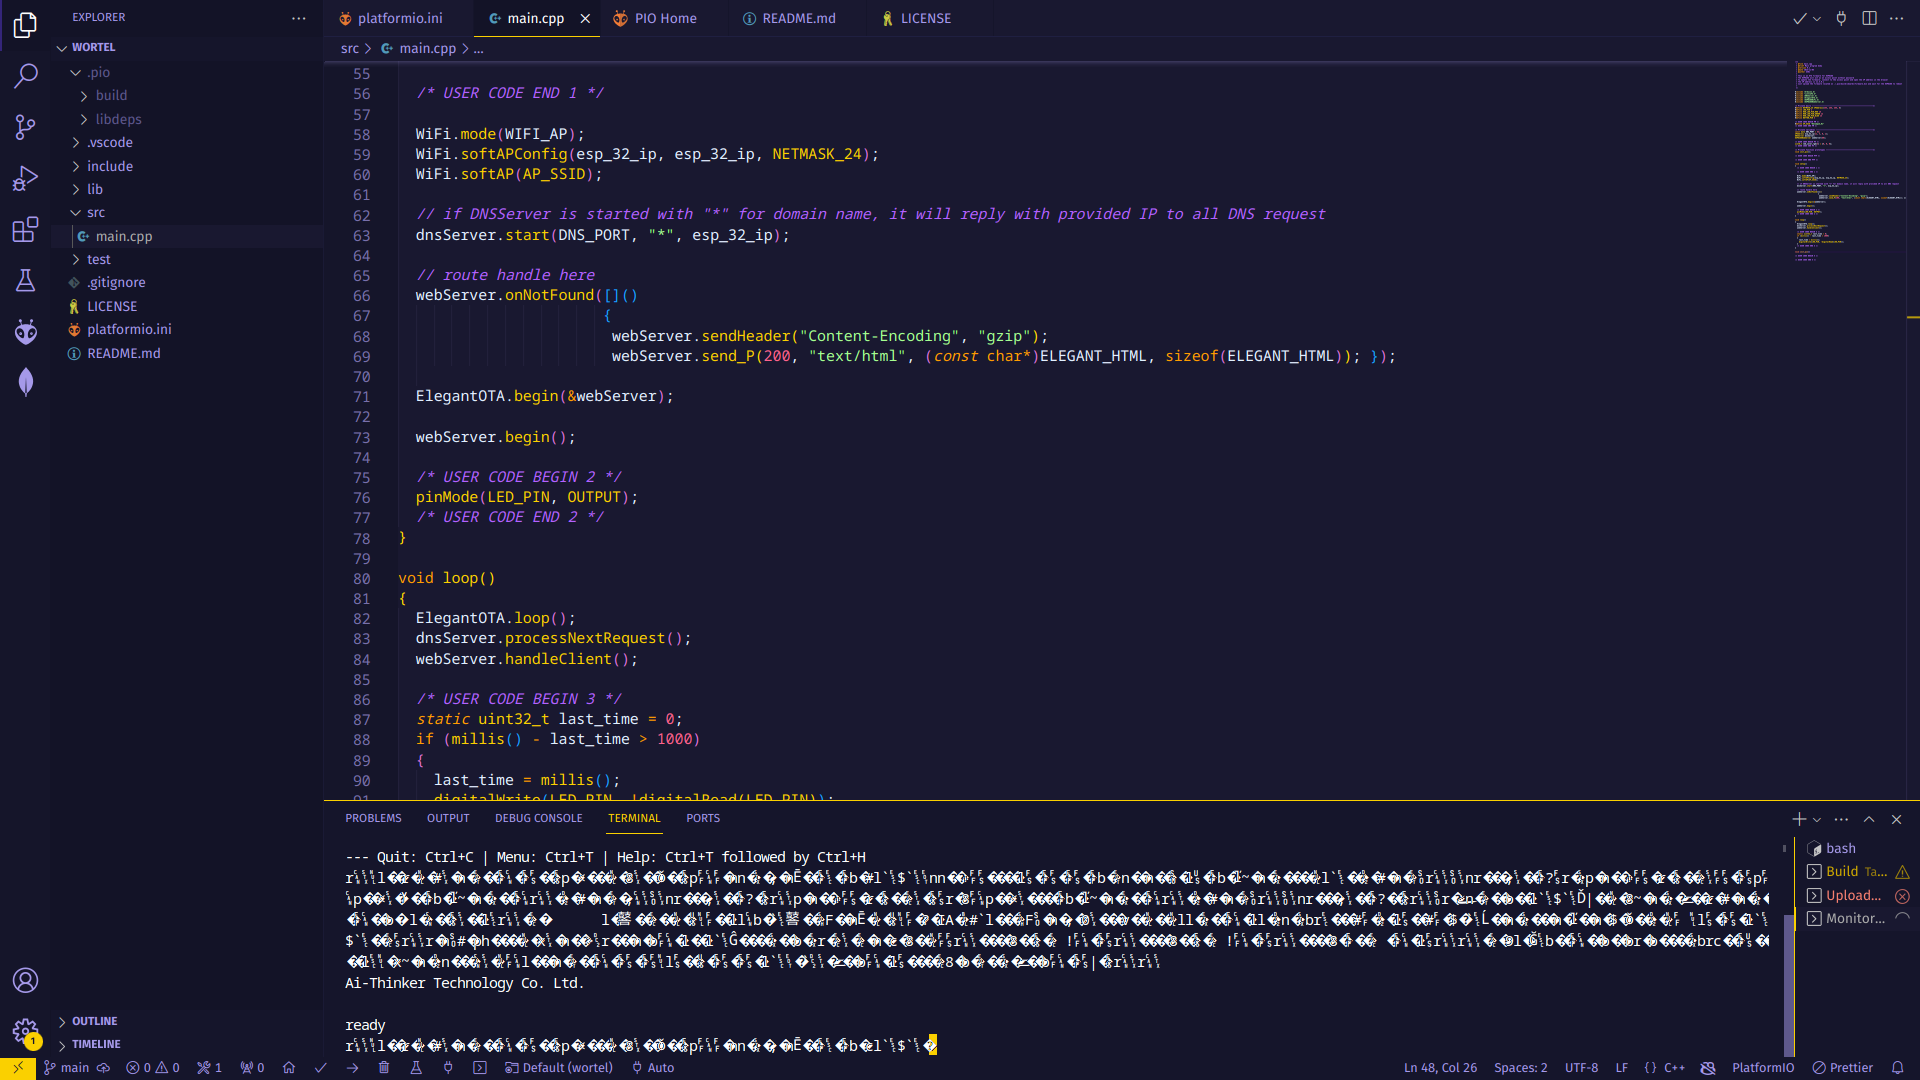
\includegraphics[width=0.4\linewidth]{P4/img/10_tampilan_ketika_esp_masuk_bootloader.png}
        \caption{Tampilan Mode Bootloader}
        \label{fig:TampilanModeBoot}
    \end{figure}
    \item Upload firmware menggunakan PlatformIO, caranya klik icon panah pada pojok kiri bawah.
    \begin{figure}[H]
        \centering
        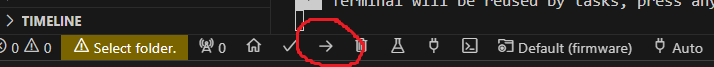
\includegraphics[width=0.4\linewidth]{P4/img/14_icon_upload_platformIO.png}
        \caption{Icon Upload PlatformIO}
        \label{fig:IconUploadPlatformIO}
    \end{figure}
    \item Tunggu hingga proses upload berhasil.
    \item Tekan tombol reset satu kali untuk menjalankan program yang telah di upload.
    \item Selanjutnya adalah uji fungsional, caranya tekan tombol boot dengan variasi sebagai berikut:
    \subitem - tekan sekali, lalu cek warna rgb nya.
    \subitem - tekan sekali lagi, lalu cek warna rgb nya.
    \subitem - tekan tahan, lalu cek warna rgb nya.
    \subitem - tekan dua kali, lalu cek warna rgb nya.
    \subitem - tekan tiga kali, lalu cek warna rgb nya.
    \item Tulislah analisisnya pada laporan serta cocokkan dengan kode pada main.cpp untuk mendukung analisis tersebut.
    \item Dokumentasikan hasil.
\end{enumerate}